\section{Methods}
\label{sec: Methods}

This section provides the details regarding the implementation of the automated analysis of Fair Use cases, particularly in data representation and the retrieval process.

\begin{figure}[h]
    \centering
    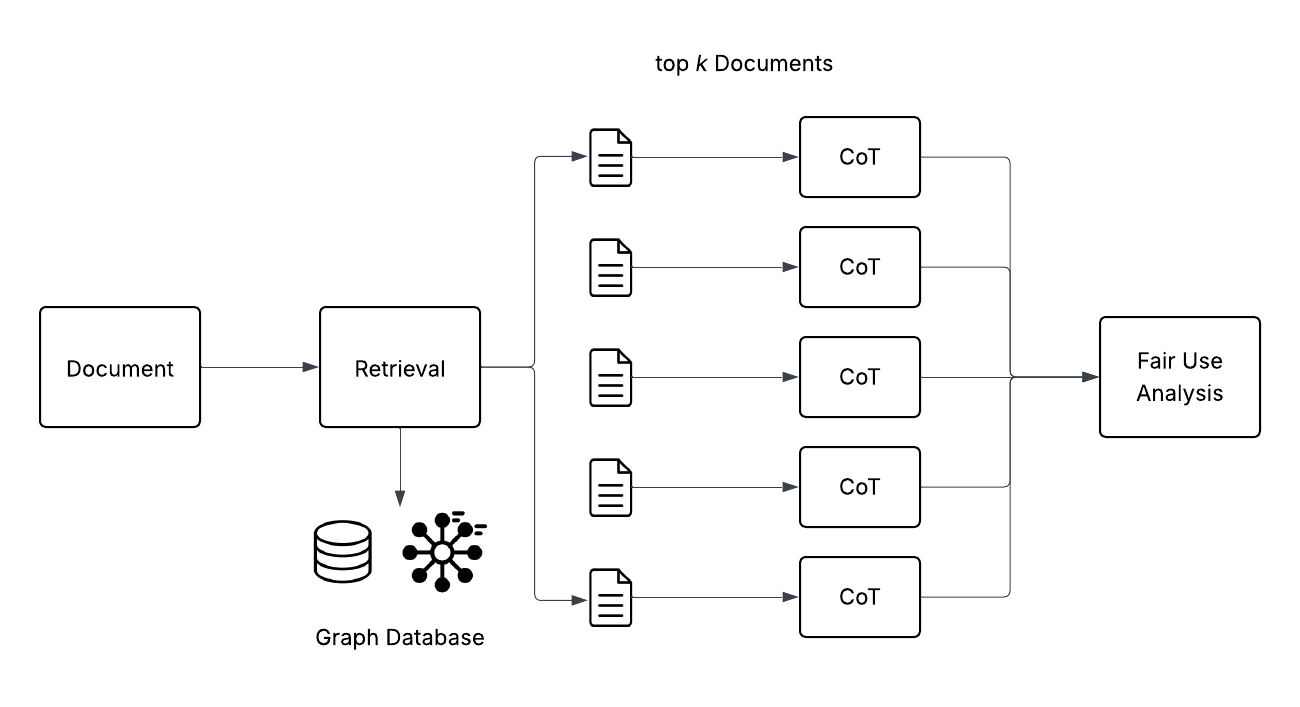
\includegraphics[width=\linewidth]{FairUseAnalysis.png}
    \caption{Overview of the Automated Analysis of Fair Use Cases.}
    \label{fig:fair_use_legal_bot}
\end{figure}

Figure \ref{fig:fair_use_legal_bot} shows an overview
of the methods used, beginning with the provided document by the user, then the retrieval step to the graph database, followed by evaluating the top-\textit{k} documents using Chain-of-Thought reasoning prior to the final inference that produces the Fair Use Analysis. The prompts used for CoT can be found in the \href{https://github.com/justinhjy1004/FairUseLegalBot/blob/main/RetrievelTesting/evaluator.py}{GitHub repository}.

The Large Language Model used is Google's Gemini Flash 2.0 \cite{11_GeminiLLM}, and the embedding model for semantic-based vector search is Google's Gecko \cite{29_GeckoEmbeddings}.

\subsection{Data Corpus}

We identified all legal precedents relevant to the Fair Use Doctrine in copyright by searching for the keywords: [keywords here...] via WestLaw Case Search. We then sourced the legal corpus relevant to the Fair Use Doctrine in copyright from Court Listener \cite{25_free_law_project_recap_2020} and [the other source here]. Furthermore, we used EyeCite, an Open Source Software developed to identify case law citations in documents to construct our citation network \cite{24_eyecite}. 

\begin{table}[h!]
  \centering
  \caption{Corpus Overview}
  \begin{tabular}{lc}
    \toprule
    Total Number of Cases & 209 \\
    Total Number of Opinions & 283 \\
    Time Range Coverage & 1976-2025\\
    Number of Unique Courts & 51 \\
    \bottomrule
  \end{tabular}
\end{table}

The number of opinions exceeds the number of cases because a single case may generate multiple judicial opinions, including appellate decisions, as well as concurring or dissenting views authored by individual judges.

Additionally, we sourced complaints related to Copyright infringement that were not resolved in court from Public Access to Court Electronic Records (PACER) \cite{26_PACER}. These serve as a preliminary test dataset for our working prototype, as they represent real Fair Use disputes that were unresolved, and hence provide a way to measure how well our model performs in unresolved cases.

We sourced a total of [number of cases here], and they were identified by [how they were obtained/searched].

\subsection{Data Representation}
\label{sec: data_representation_KG}

Our knowledge graph is implemented using Neo4j \cite{27_neo4j}. In order to more faithfully represent the data in Legal Precedents related to the Fair Use Doctrine in Copyright, we modeled the cases with a knowledge graph as depicted in Figure \ref{fig:KG_Schema}. This incorporates important features of the legal system in the United States where legal precedents issued by a higher court have higher authority over others, as well as the citation network formed between the cases.

Furthermore, in every given opinion, we extract the verbatim paragraphs related to the \textit{Facts} of the case, the four factors: (1) \textit{Purpose} and character of the use (2) \textit{Nature} of the copyrighted work, (3) \textit{Amount} and substantiality of the portion used, and (4) Effect of the use on the Potential \textit{Market}. We also included the \textit{Conclusion} of the opinion to reflect how the court balanced the four factors to arrive at their opinion. The extraction is done using the LLM to identify and extract verbatim paragraphs in which each of the four Fair Use factors were discussed, along with the factual background and the court's conclusion. We designed specific prompts to direct the LLM to focus on legal reasoning and factor-specific content. These prompts instruct the model to return direct quotations from the opinion text corresponding to each factor, rather than paraphrased summaries. For transparency and reproducibility, the prompts used can be found in the project’s GitHub repository. 

\begin{figure}[ht]
\centering
\begin{tikzpicture}[
    ->, >=Stealth,
    % Node style: circles, same size, white fill, black outline.
    nodeStyle/.style={
        align=center,
        font=\scriptsize,
        fill=white
    },
    % Plain edge labels: no border/circle
    labelStyle/.style={
        font=\scriptsize
    },
    scale=0.9,
    transform shape
]

%--- Top row of nodes ---
\node[nodeStyle] (courts)      at (1,-1)   {Courts};
\node[nodeStyle] (cases)       at (4,-1)   {Cases};

%--- Middle node ---
\node[nodeStyle] (opinion)     at (2.5,-2)  {Opinion};

%--- Bottom row of nodes ---
\node[nodeStyle] (facts)       at (0,-2)  {Facts};
\node[nodeStyle] (purpose)     at (1,-3) {Purpose};
\node[nodeStyle] (nature)      at (2,-4)  {Nature};
\node[nodeStyle] (market)      at (3,-4) {Market};
\node[nodeStyle] (amount)      at (4,-3)  {Amount};
\node[nodeStyle] (conclusion)  at (5,-2)   {Conclusion};

%-----------------------
%        Edges
%-----------------------
% (1) Courts -> Courts (loop): "Appeals to"
\draw[->]
  (courts) edge [loop left] node[labelStyle] {Appeals to} (courts);

% (2) Courts -> Cases: "Decided"
\draw[->] 
  (courts) -- node[labelStyle, above] {Decided in} (cases);

% (3) Cases -> Cases (loop): "Cited"
\draw[->]
  (cases) edge [loop right] node[labelStyle] {Cited} (cases);

% (4) Cases -> Opinion: "Has-opinion"
\draw[->]
  (cases) -- node[labelStyle, left] {Has opinion} (opinion);

% (5) Facts -> Opinion: "of"
\draw[->]
  (facts) -- node[labelStyle, above, sloped] {of} (opinion);

% (6) Purpose -> Opinion: "of"
\draw[->]
  (purpose) -- node[labelStyle, above, sloped] {of} (opinion);

% (7) Nature -> Opinion: "of"
\draw[->]
  (nature) -- node[labelStyle, above, sloped] {of} (opinion);

% (8) Market -> Opinion: "of"
\draw[->]
  (market) -- node[labelStyle, above, sloped] {of} (opinion);

% (9) Amount -> Opinion: "of"
\draw[->]
  (amount) -- node[labelStyle, above, sloped] {of} (opinion);

  % (9) Conclusion -> Opinion: "of"
\draw[->]
  (conclusion) -- node[labelStyle, above, sloped] {of} (opinion);
\end{tikzpicture}
\caption{Domain Specific Knowledge Graph Schema of Judicial Opinions of the Fair Use Doctrine in Copyright 17 U.S. Code § 107.}
\label{fig:KG_Schema}
\end{figure}

The choice of our data representation is that it is not only a more faithful representation of the data, which allows us to use the structure of the data (i.e. citations) to improve our retrieval process, but it also provides the ability to retrieve based on contextual similarity. For instance, a complaint on Copyright Infringement might be similar with respect to the medium in which the work was distributed (print or via video recordings), but might differ substantially based on the Purpose of the use (ie. Parody, Criticism or for Educational Reasons). 

The choice of using a Knowledge Graph representation allows for more granular, context-specific similarity comparison during the retrieval process which has shown to be effective \cite{02_DenseRetrieval, 03b_SemanticRepresentationContextual}. Moreover, the interpretability of such representation might increase the interest, trust, and therefore adoption of LLMs in the legal space since this mimics how legal experts might reason in the context of Fair Use \cite{18_TrustAIExplainability}.

Each case is modeled as a node connected to its issuing court and to the legal opinion(s) it contains. Opinions are linked to factor-specific paragraph nodes (e.g., Purpose, Market, Nature), enabling granular retrieval by legal reasoning dimensions. Citations between cases form directed edges within the graph. The schema is implemented in Neo4j using labeled nodes (e.g., \texttt{Case}, \texttt{Court}, \texttt{Opinion}, \texttt{Fact}) and relationship types (e.g., \texttt{DECIDED\_IN}, \texttt{HAS\_OPINION}, \texttt{CITED}, \texttt{APPEALS\_TO}). This representation supports both structural queries (e.g., retrieving appellate court opinions) and vector search via LLM embeddings.

\subsection{Retrieval and Reranking}

Our retrieval process combines semantic-based vector search by computing similarity scores. However, we extend this by incorporating two features from the data representation by determining the authoritativeness of a legal precedent using the \texttt{PageRank} algorithm as well as the cited opinions of the opinions that were retrieved.

As discussed in Section \ref{sec: data_representation_KG}, the verbatim passages that discuss the facts of the case, the four factors of Fair Use, and the conclusion of the case were extracted using an LLM. We then chunk the passages and embed them using \texttt{Gecko}. We use cosine similarity as our method in computing the similarity between the documents. Furthermore, to incorporate the citation metrics as well as the court hierarchy, we used the PageRank algorithm to quantify the relative importance of each court decision within the legal citation network. This is done for both the legal opinions (based on the citations) and the courts (based on appellate relationships). 

We used the PageRank algorithm to quantify two distinct but complementary aspects of legal authority: citation authority, calculated from the inter-opinion citation network, and court hierarchy, based on appellate relationships among courts. While these dimensions capture different sources of legal relevance—influence through citation versus institutional authority by position in the judiciary, they are often correlated in practice, as higher courts tend to issue opinions that are more frequently cited. However, we include this dual representation to allow our model to consider both the structural and reputational weight of each legal source.

The retrieved documents are ranked based on a convex combination, where
\begin{equation}
    s_{i} = w_{\text{text}}\text{TextSim}_i + w_{\text{cit}}\text{Citation}_i + w_{\text{court}}\text{Court}_i
\end{equation}
such that $w_{\text{text}}, w_{\text{cit}}, w_{\text{court}} \in [0,1]$ and $w_{\text{text}} + w_{\text{cit}} + w_{\text{court}} = 1$. The weights hence can be interpreted as hyperparameters in which one can adjust for optimal retrieval. We applied \texttt{min-max} scaling the scores individually to ensure that each score is between 0 and 1. In the current prototype, the weights are manually specified by the user, which allows legal experts to adjust the retrieval behavior based on the characteristics of the query or dispute. For instance, a researcher may prioritize citations and court hierarchy in appellate-heavy disputes, while another may favor textual similarity in novel or atypical cases. In future work, we plan to systematically evaluate the effect of different weight configurations using ablation studies.

Lastly, based on the top $k$ legal precedents that are retrieved, an additional parameter $n$ can be specified to retrieve the cited opinions by the retrieved cases based on the citation and court rankings. These cited cases are included directly in the inference step to provide broader legal context and to simulate how a legal practitioner might draw from precedent when reasoning about a novel dispute.

\begin{figure}[h]
    \centering
    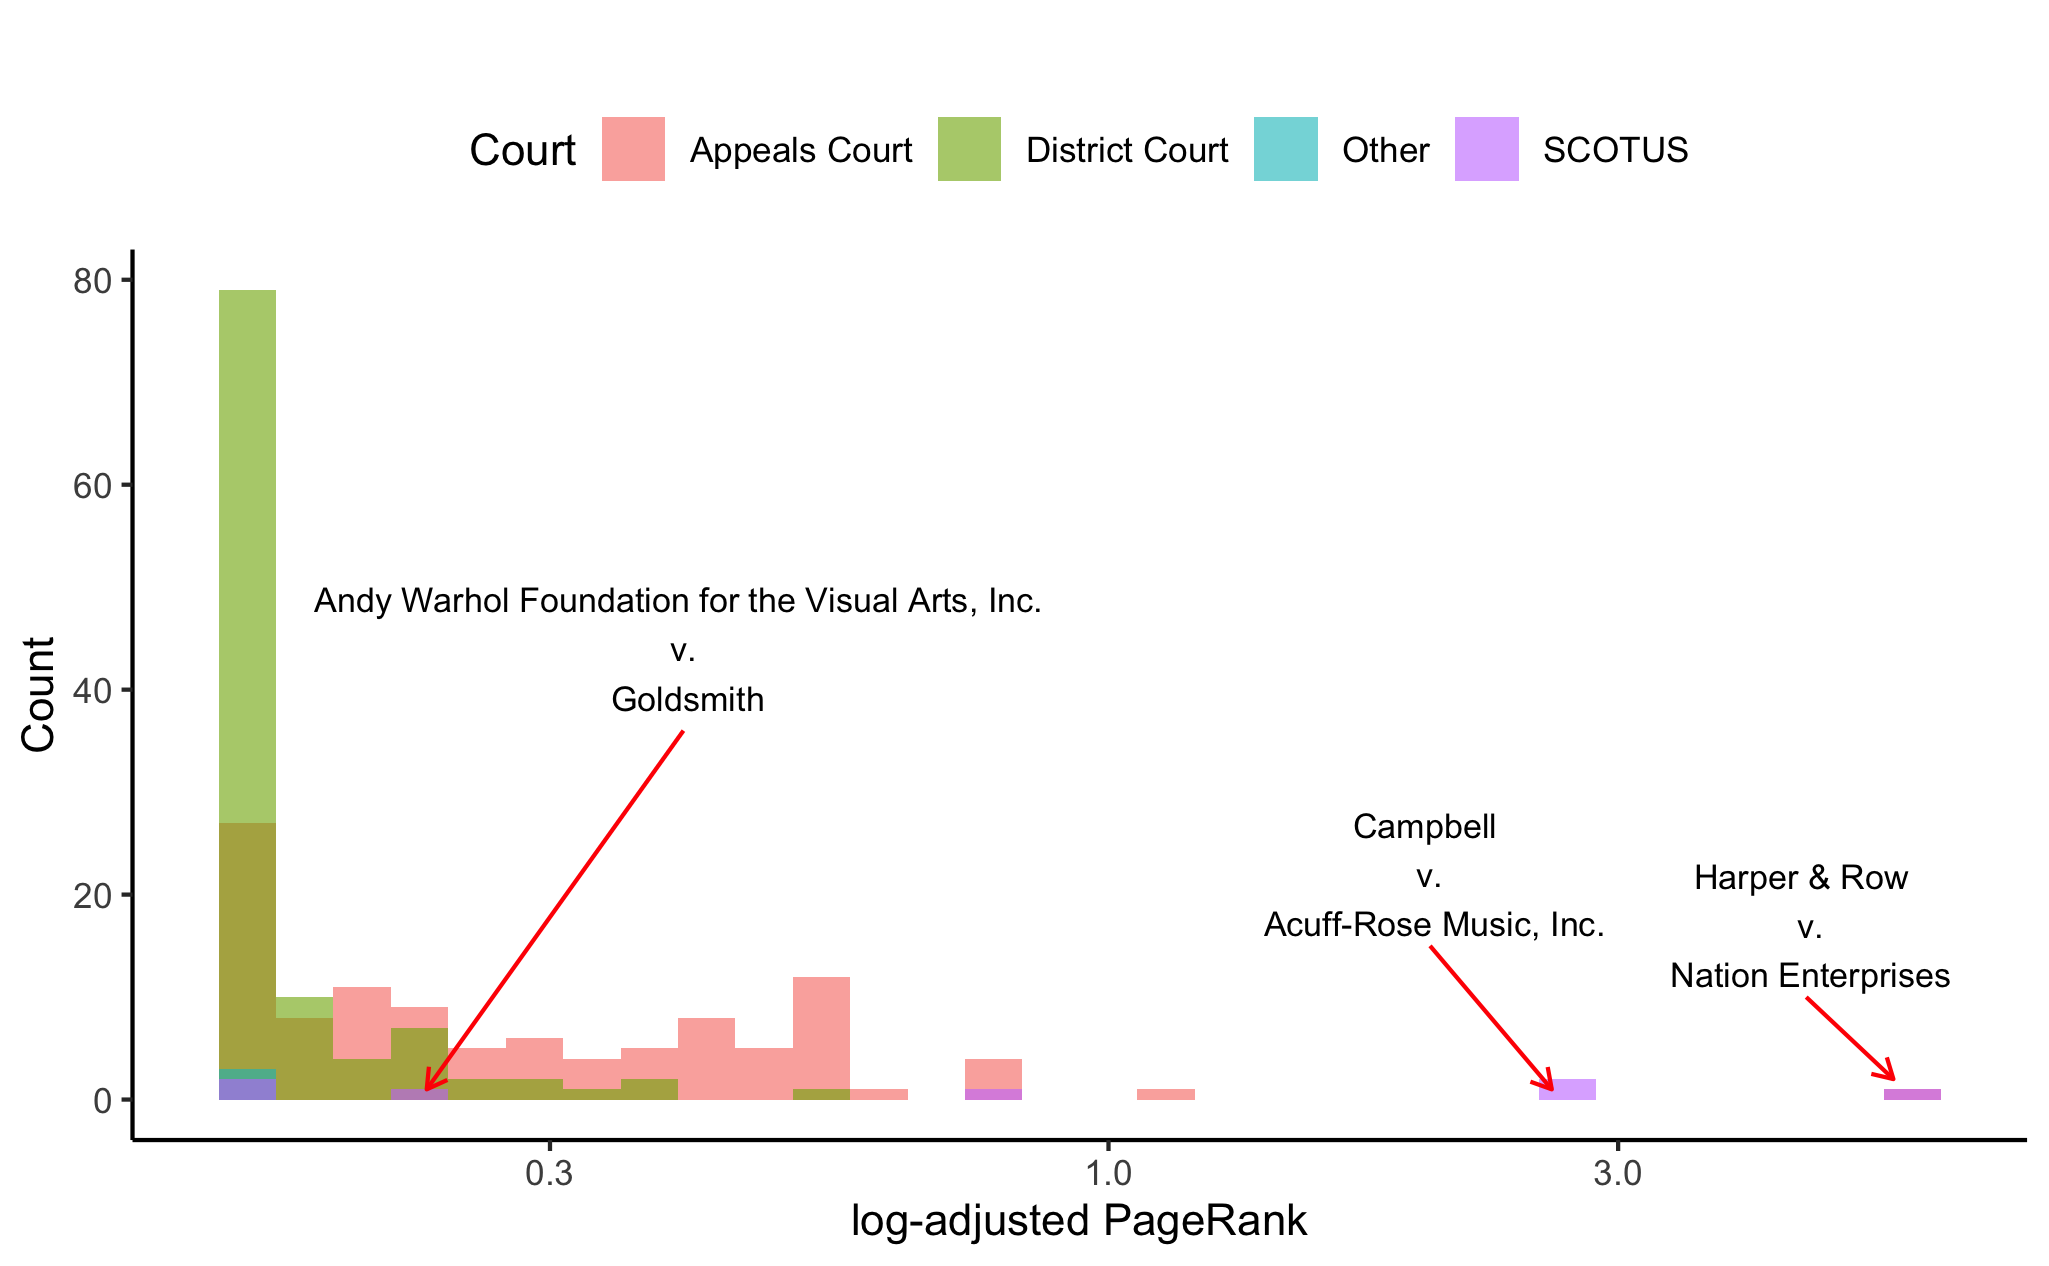
\includegraphics[width=\linewidth]{histogram_pagerank.png}
    \caption{Distribution of Legal Case Influence by Court and PageRank}
    \label{fig:pagerank}
\end{figure}

Figure \ref{fig:pagerank} displays the distribution of legal cases by their log-adjusted PageRank, a measure of influence within the legal citation network. Most cases, particularly from District Courts, cluster at lower PageRank values, while a few landmark Supreme Court decisions like \textit{Campbell v. Acuff-Rose Music, Inc.} and \textit{Harper \& Row v. Nation Enterprise} have disproportionally high PageRank values. This is, of course, not surprising, as many natural networks exhibit power-law distributions \cite{33_ScaleFreeNetwork}.

Although the \textit{Warhol v. Goldsmith} case is considered to be highly significant by most legal scholars, its recency means it has had limited time to accumulate citations. This is a limitation of PageRank which does not account for time. Future work could explore time-adjusted measures to better capture the emerging influence of newer cases.

\subsection{Current Progress and Implementation}

\begin{figure}[h]
    \centering
    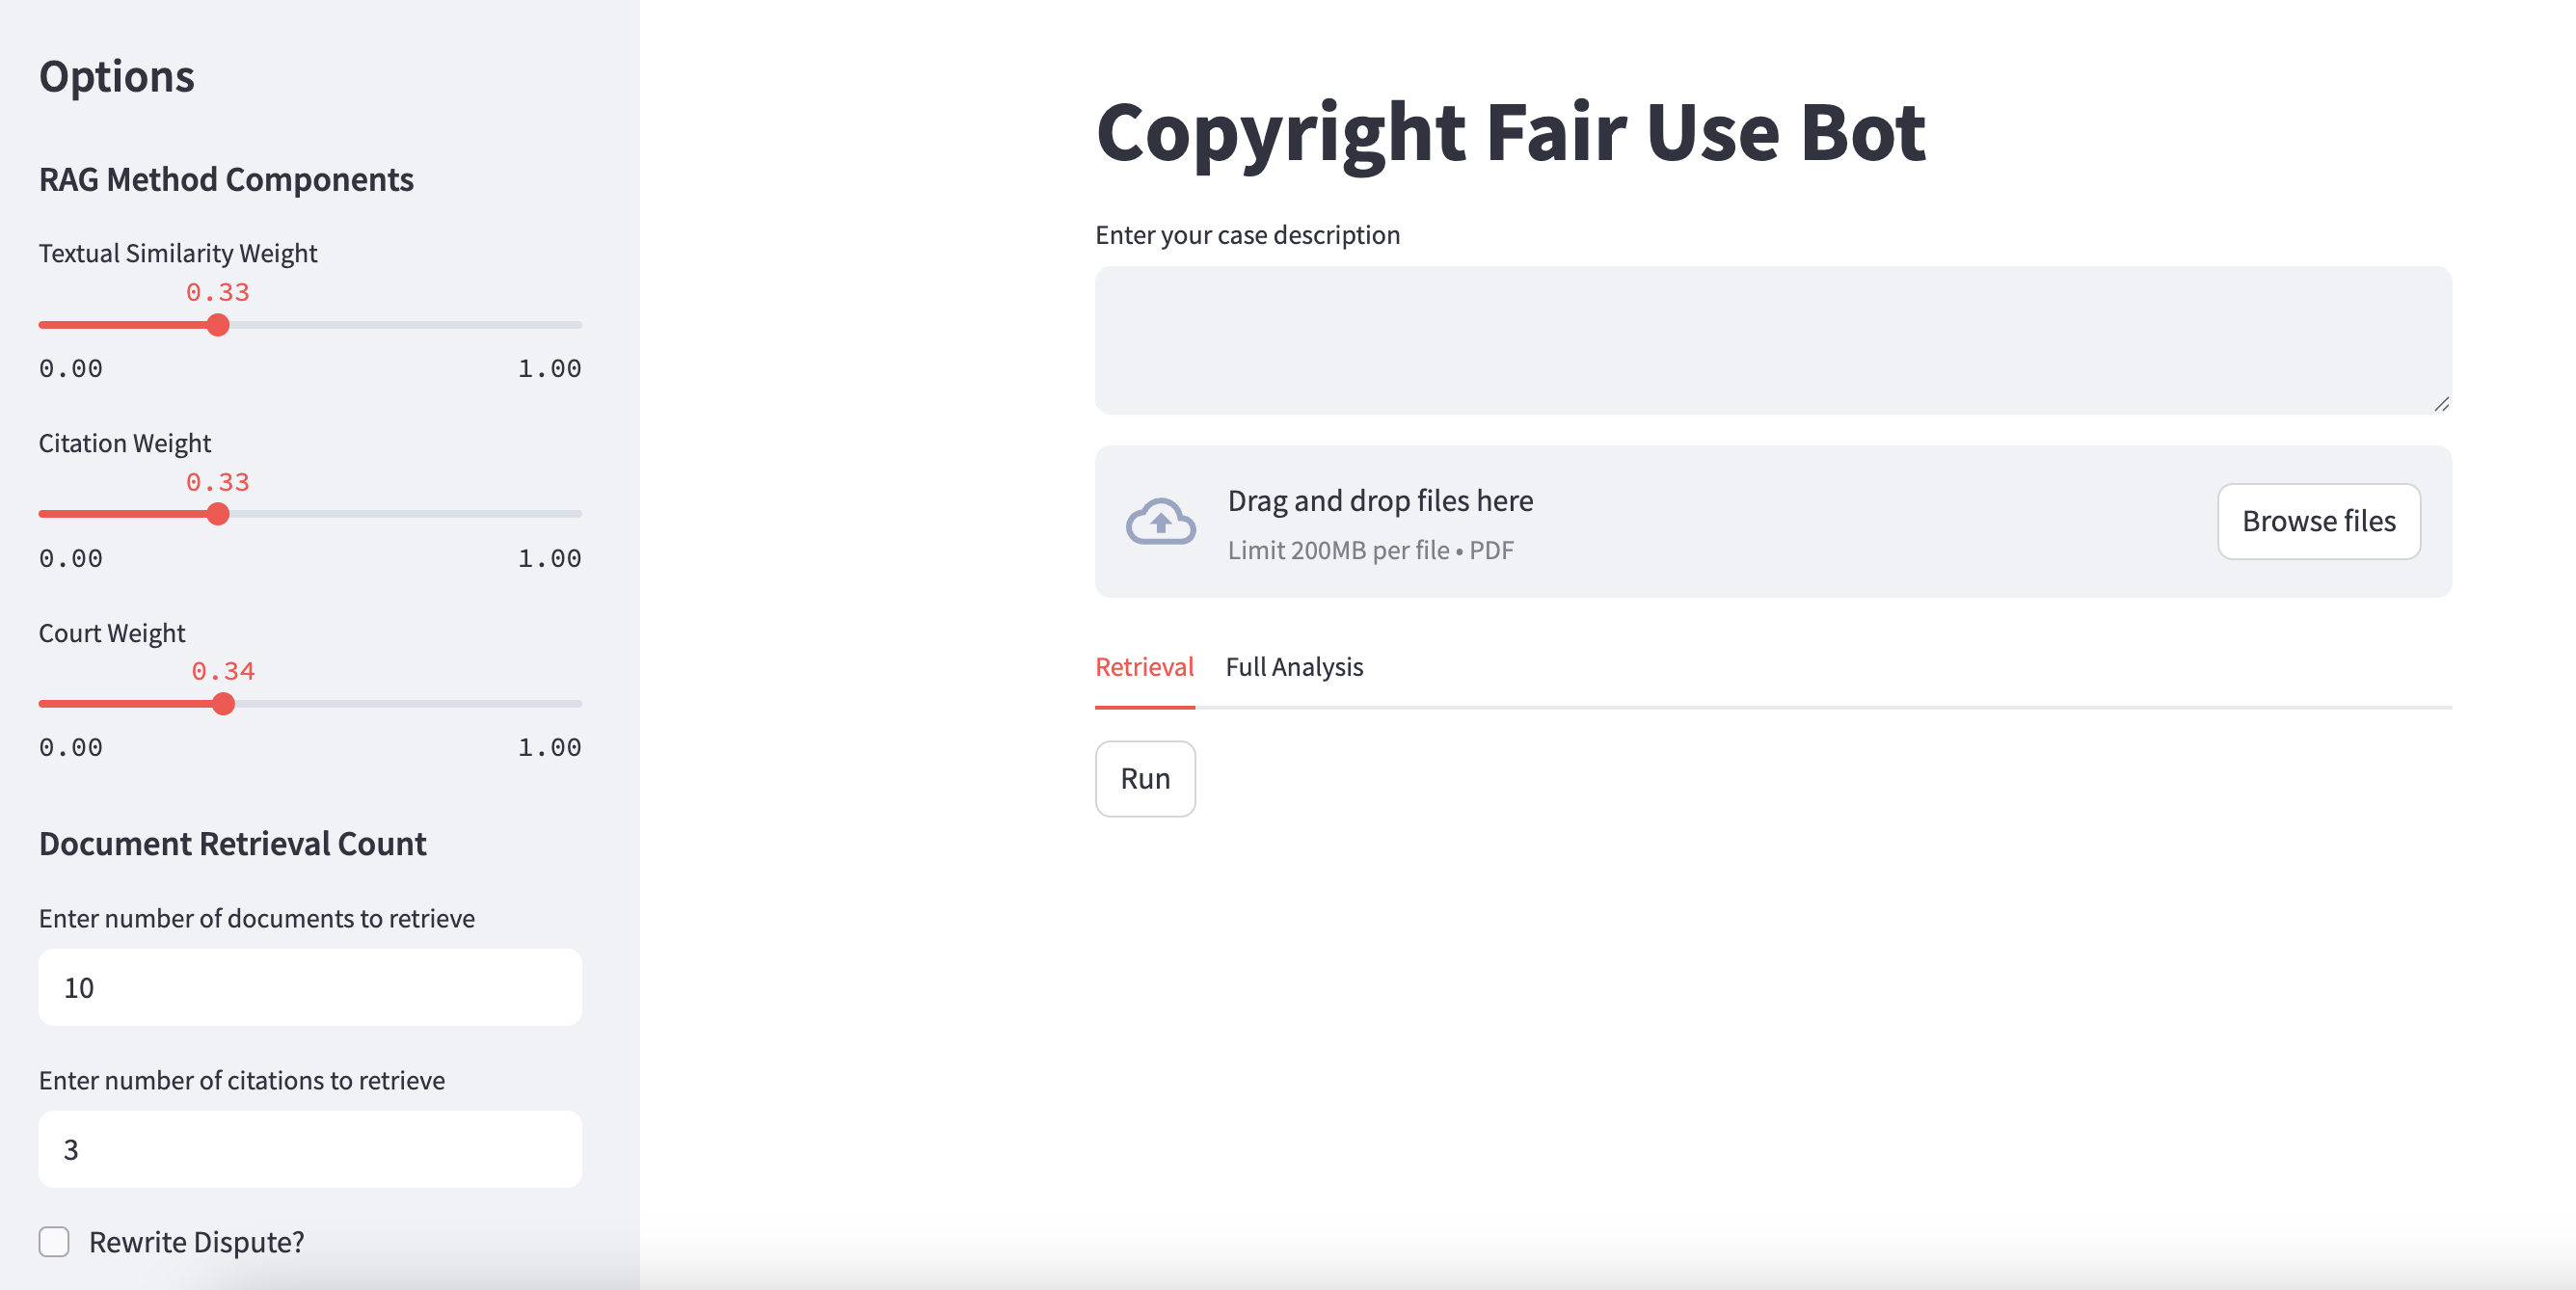
\includegraphics[width=\linewidth]{Interface.png}
    \caption{Interface of the Fair Use Legal Bot}
    \label{fig:interface}
\end{figure}

As of April 2025, we have developed a functional prototype of the application. The current prototype of the Fair Use Legal Bot can be found \href{https://fairuselegalbot-main.streamlit.app/}{here}. Figure \ref{fig:interface} shows the interface where users can provide their case or dispute description for fair use analysis. Users can upload relevant documents in PDF format or enter a written description directly into the input box. They can also customize the retrieval algorithm by adjusting the weights for textual similarity, citation frequency, and court relevance, as well as specify the number of documents and citations to retrieve. This prototype was developed mainly for internal testing and refinement of the retrieval process, but is accessible to external users for testing and evaluation.

The current version supports uploading a complaint or a text description of a dispute, and retrieve the most relevant documents based on the hyperparameters configured in the left panel (``RAG Component Methods”). We have currently implemented the manual weighting of the three parameters, and users can specify the $k$ number of documents as well as $n$ number of cited cases. 

While formal evaluations and user studies have not yet been conducted, the current version of the application establishes a strong foundation for future experimentation and ablation studies. Preliminary testing of the retrieval system is presented in the following section. Internally, the application has been tested on [data size/type], with early feedback from [users/testers] indicating that [brief takeaway].
